\documentclass[a4paper, 12pt]{article}
\usepackage{graphicx} % Required for inserting images
\usepackage{textcomp}
\usepackage{fullpage}
\usepackage{amsmath}
\usepackage{xcolor}
\usepackage{float}
\usepackage{geometry}
\usepackage{biblatex}
\geometry{margin=1in}
\usepackage{enumitem}
\usepackage{hyperref}
\usepackage{microtype}
\usepackage{gensymb}
\usepackage{parskip}
\usepackage{tikz}
\usepackage{caption}
\usepackage{cancel}
\usepackage{nicefrac}
\hypersetup{
    colorlinks=true,        % Enable colored links
    linkcolor=teal,         % Set color for internal links
    citecolor=teal,         % Set color for citations
    filecolor=teal,         % Set color for file links
    urlcolor=teal           % Set color for URLs
}

\usepackage[version=4]{mhchem}

\newcommand{\degC}{$\degree$C \,}
\newcommand{\degF}{$\degree$F \,}
\newcommand{\R}{\left(0.0821 \: \frac{L \cdot atm}{mol \cdot \text{K}}\right)}
\newcommand{\cunits}{$\frac{J}{g \degree \text{C}}$}

\title{Chem Honors Study Guide 5}
\author{Test 2 S2}
\date{Test date: March 28}

\begin{document}

\maketitle

\section{Serial Dilution}
A serial dilution is a series of multiple dilutions in a row.

\subsection*{Dilution Steps}

\begin{enumerate}[leftmargin=*]
    \item Take 1 $ml$ of the original solution and add it to a second container.
    \item Add $x-1 \: ml$ of water.
    \item Repeat as many times as necessary. The molarity should have decreased by $x$ times (e.g. if you are performing a $1:4$ dilution and the original molarity was 1.0 $M$, the molarity after diluting once is 0.25 $M$).
\end{enumerate}

\subsection*{Beer's Law}

\begin{equation}\label{beers}
A = \varepsilon l c
\end{equation}
where:
\begin{itemize}[leftmargin=*, nosep]
    \item $A$ is the absorbance
    \item $\varepsilon$ is the molar absorptivity (slope)
    \item $l$ is the pathlength
    \item $c$ is the concentration
\end{itemize}

\section{States of Matter}

\subsection*{Three States of Matter}

\begin{table}[H]

\begin{tabular}{c|c|c|c}
\textbf{State of Matter} & \textbf{Conforms?} & \textbf{Closely packed?} & \textbf{Compressible?} \\\hline
solid & no & yes & no \\
liquid & yes & yes & no \\
gas & yes & no & yes
\end{tabular}

\vspace{1em}
Solids are not always more closely packed than liquids! There are exceptions, such as water.

\end{table}

\subsection*{Temperature}
Kelvin K Fahrenheit \degF Celsius \degC

$$\degree \text{F} = 1.8(\degree\text{C}) + 32$$
$$\degree \text{C} = \frac{\degree \text{F} -32}{1.8}$$
$$\text{K} = \degree\text{C} + 273$$
$$\degree\text{C} = \text{K} - 273$$
$$\Delta T \: (\text{in} \degree\text{F}) = 1.8 \cdot \Delta T \: (\text{in} \degree\text{C or K})$$

\subsection*{Kinetic Energy}
\begin{equation}\label{ke}
    \text{KE} = \frac{1}{2}mv^2
\end{equation}

Example: Which gas would move 4x faster than O$_2$?

Solution: Using \ref{ke}:

$$\frac{1}{2}(32 \: g/mol)(1 \: \text{(arbitrary unit of velocity))} = \frac{1}{2}(x \: g/mol)(4)$$
$$x = 2$$
$$\boxed{\text{H}_2}$$

\section{Gasses}

\subsection*{Definitions}

\begin{itemize}[leftmargin=*, nosep]
    \item \textbf{\textit{gas pressure}}: Collisions of molecules with the container.
    \item \textbf{\textit{diffusion}}: The movement of particles from high concentration to low concentration until the concentration is consistent throughout.
    \item \textbf{\textit{effusion}}: The movement of particles through a small hole in the container.
    \item \textbf{\textit{long-range order}}: A regular, repetitive arrangement of particles. Solids with long-range order are called crystalline, and those without are called amorphous.
    \item \textbf{\textit{vapor pressure}}: Measure of the tendency of a liquid to vaporise.
\end{itemize}

\subsection*{Pressure Units}
760 $mm$Hg (millimeters of mercury) = 1 $atm$ (atmosphere)

\subsection*{The Gas Laws}
where:

\begin{itemize}[leftmargin=*, nosep]
    \item $P$ is the pressure
    \item $V$ is the volume
    \item $T$ is the temperature \textbf{in Kelvin}
    \item $n$ is the number of moles
    \item $R$ is the ideal gas constant equal to 0.0821
\end{itemize}

\begin{equation}\label{boyle}
    \text{\textbf{Boyle's Law: }}P_1V_1 = P_2V_2
\end{equation}
\begin{equation}\label{charles}
    \text{\textbf{Charles' Law: }}\frac{V_1}{T_1} = \frac{V_2}{T_2}
\end{equation}
\begin{equation}\label{gaylussac}
    \text{\textbf{Gay-Lussac's Law: }}\frac{P_1}{T_1} = \frac{P_2}{T_2}
\end{equation}
\begin{equation}\label{combined}
    \text{\textbf{Combined Gas Law: }}\frac{P_1V_1}{T_1} = \frac{P_2V_2}{T_2}
\end{equation}
\begin{equation}\label{avogadro}
    \text{\textbf{Avogadro's Law: }}\frac{V_1}{n_1} = \frac{V_2}{n_2}
\end{equation}
\begin{equation}\label{ideal}
    \text{\textbf{Ideal Gas Law: }}PV = nRT
\end{equation}

\paragraph{Important:}

\begin{itemize}[leftmargin=*, nosep]
    \item $P \propto T$ and $V \propto T$. $P \propto \frac{1}{V}$. (P and V are directly proportional to T, and P is proportional to the reciprocal of V or inversely proportional to V.)
    \item Always use K for temperature.
    \item Laws \ref{boyle}, \ref{charles}, and \ref{gaylussac} are only true \textbf{if the temperature, pressure, and volume are held constant.}
    \item The ideal gas law uses specific units. The constant $R$, 0.0821, uses the units $\frac{L \cdot atm}{mol \cdot \text{K}}$, so volume must be in $L$, pressure in $atm$, and, as always, temperature in K.
    \item STP (standard temperature and pressure) is at 0\degC or 273K when 1 $mol$ of any gas occupies 22.4 $l$.
\end{itemize}

Example: The density of an unknown gas at 20\degC and 749 $mm$Hg is 1.31 $g/L$. Calculate the molar mass of the gas.

Solution: Using \ref{ideal}, assuming 1 $L$ of the gas, and converting to proper units:

$$(0.986 \: atm)(1 \: L) = \R (293\text{K})(n)$$
$$n = 0.041 \: mol$$
$$1.31 \: g \div 0.041 \: mol$$
$$=\boxed{32.0 \: g/mol}$$

\subsection*{Diffusion and Effusion}

\subsubsection*{Law of Effusion}

\begin{equation}\label{effusion}
    \frac{\text{rate}_A}{\text{rate}_B} = \sqrt{\frac{\text{MM}_B}{\text{MM}_A}}
\end{equation}

where MM denotes molar mass.

Example: How many times faster does He effuse than N$_2$?

Solution: Using \ref{effusion}:

$$\frac{\text{rate}_\text{He}}{\text{rate}_\text{N$_2$}} = \sqrt{\frac{28.014}{4.003}}$$
$$=\boxed{2.65}$$

Example: Which gas diffuses 2.23 times faster than Br$_2$?

$$2.23 = \sqrt{\frac{159.808 \: g/mol}{x}}$$
$$x \approx 32 \: g/mol$$
$$\boxed{\text{O}_2}$$

\subsubsection*{Other Formulas}

\begin{equation}\label{totalpressure}
    \text{\textbf{Total pressure: }} P_{\text{total}} = P_A + P_B + P_C + \cdots
\end{equation}
The total pressure of a mixture of gasses is equal to the sum of the pressures of its constituent parts.

\begin{equation}\label{molefraction}
    \text{\textbf{Definition of the mole fraction: }} \chi_a = \frac{n_A}{n_\text{total}}
\end{equation}
The mole fraction is defined as the number of moles of a substance over the moles of total gas.

\begin{equation}\label{partialpressure}
    \text{\textbf{Dalton's Law of Partial Pressure: }} P_a = \chi_a \cdot P_{\text{total}} 
\end{equation}
The pressure exerted by an individual gas is equal to the mole fraction times the total pressure.

Example: If you have 2.1 $mol$ N$_2$, 0.8 $mol$ CO$_2$, and 0.3 $mol$ O$_2$ at 297K and occupying 1.8 $L$, what is $P_{\text{total}}$ and the partial pressures?

\textcolor{blue}{\textbf{Step 1:} Add the number of moles together.}

$$2.1 + 0.8 + 0.3 = 3.2 \: mol$$

\textcolor{blue}{\textbf{Step 2:} Use $PV = nRT$} to find the total pressure.

$$PV = nRT$$
$$(1.8 \: L)(P) = \R (3.2 \: mol)(297\text{K})$$
$$P = 43.35 \: atm$$

\textcolor{blue}{\textbf{Step 3:} Find the mole fractions} for each element with \ref{molefraction}.

$$\chi_{\text{N}_2} = \frac{2.1 \: mol}{3.2 \: mol} = 0.656$$
$$\chi_{\text{CO}_2} = \frac{0.8 \: mol}{3.2 \: mol} = 0.25$$
$$\chi_{\text{O}_2} = \frac{0.3 \: mol}{3.2 \: mol} = 0.09$$

\textcolor{blue}{\textbf{Step 4:} Solve for partial pressure} with \ref{partialpressure}.

$$P_{\text{N}_2} = 0.656 \cdot 43.35 = 28.44 \: atm$$
$$P_{\text{CO}_2} = 0.25 \cdot 43.35 = 10.84 \: atm$$
$$P_{\text{CO}_2} = 0.09 \cdot 43.35 = 3.90 \: atm$$

$$\boxed{P_{\text{N}_2} = 28.44 \: atm; P_{\text{CO}_2} = 10.84 \: atm; P_{\text{O}_2} = 3.90 \: atm.}$$

\subsubsection*{Phase Diagrams}
Below are the phase diagrams for typical material and water:\footnote{https://byjus.com/chemistry/phase-diagram-of-water/}

\begin{figure}[H]
\centering
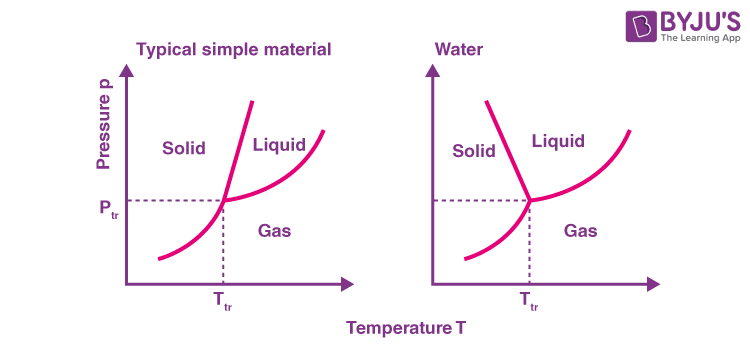
\includegraphics[width=0.7\textwidth]{phasediag.png}
\end{figure}

Note that in water, increasing the pressure leads to a phase change, since ice is less dense than water. The center point where all three lines intersect is called the \textbf{triple point}.

\subsubsection*{Melting Points of Solids}
\textbf{Distinct melting point} (H$_2$O, metals...) v. \textbf{MP range} (fats, glass, plastic, rubber...)

Solids with distinct melting points are \textbf{crystalline} solids with long-range order. Solids with a melting point range are \textbf{amorphous} solids without long range order that melt at multiple temperatures.\footnote{https://elibraryportal.com/amorphous-and-crystalline-solids/}

\begin{figure}[H]
\centering
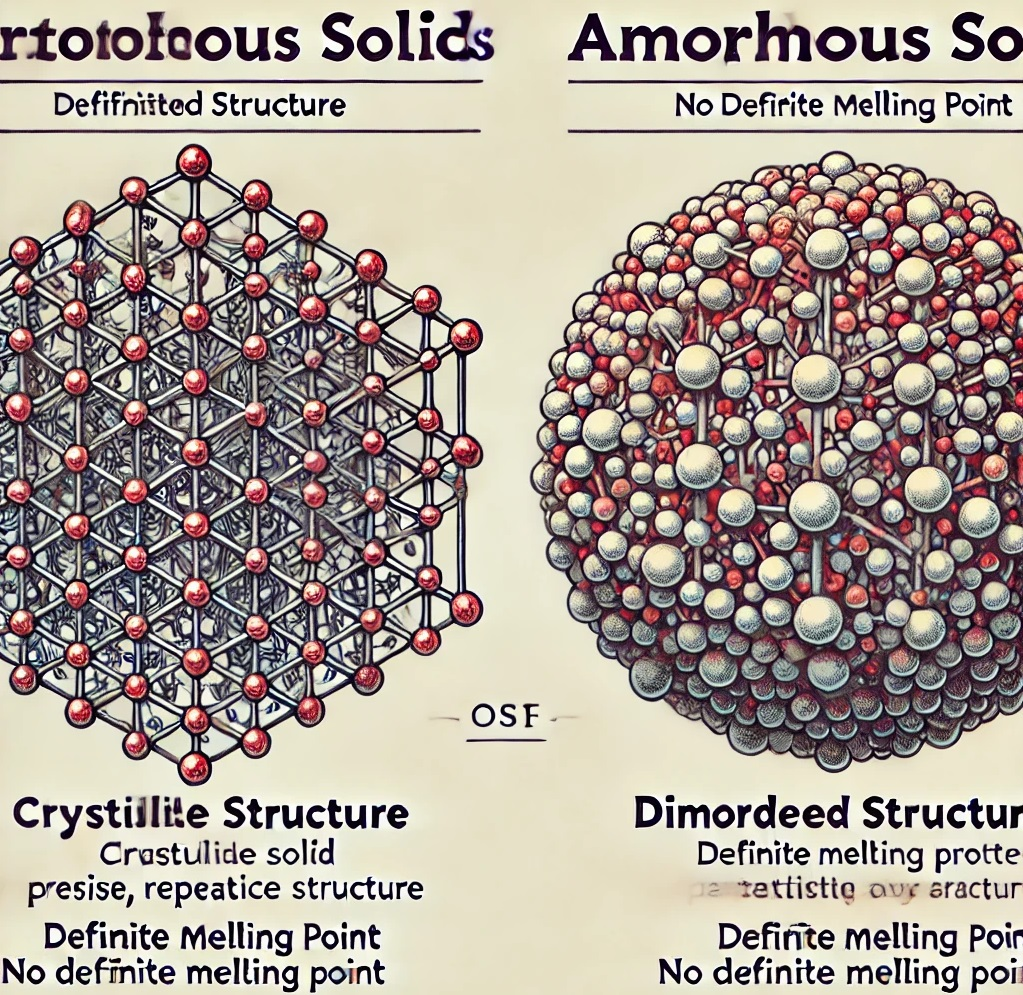
\includegraphics[width=0.5\textwidth]{funnypic.jpg}
\caption*{This is somewhat irrelevant, but here is an amusing AI-generated picture that attempts to explain this concept. (They tried.)}
\end{figure}

\subsubsection*{Vapor Pressure}
As temperature increases, vapor pressure will also increase until vapor pressure is equal to the atmospheric pressure (i.e. the boiling point). There is an exchange of molecules happening at the surface of a liquid, and if you seal the container, it will eventually reach equilibrium.

\subsubsection*{Solutions}
\textbf{Freezing point depression} happens when a non-volatile solute is added to a solvent that disrupts the lattice, interfering with the solvent's ability to form its regular crystalline structure.

\textbf{Boiling point elevation} happens when a non-volatile solute is added to a solvent and blocks the solvent from evaporating.

\section{Thermodynamics}
\subsection*{Definitions}

\begin{itemize}[leftmargin=*, nosep]
\item \textbf{\textit{heat}}: The kinetic energy of particles.
\item \textbf{\textit{temperature}}: The measurement of heat.
\item \textbf{\textit{endothermic process}}: A process that absorbs heat from surroundings, going from a lower energy state to a higher energy state.
\item \textbf{\textit{exothermic process}}: A process that releases heat into surroundings, going from a higher energy state to a lower energy state.
\item \textbf{\textit{calorie}}: The amount of energy it takes to raise 1 gram of water by 1 degree Celsius (specific heat capacity of water).
\item \textbf{\textit{specific heat capacity}}: The amount of energy it takes to raise the temperature of 1 gram of a substance by 1 degree Celsius. (For water, the specific heat capacity is 1 calorie.)
\item \textbf{\textit{bond energy}}: The heat required to break a bond or released when the bond is made.
\end{itemize}

\subsection*{Laws of Thermodynamics}

\begin{enumerate}[leftmargin=*, nosep]
\item \textbf{Energy cannot be created nor destroyed.}
\item \textbf{Heat disperses until equal.}
\end{enumerate}

\subsection*{Reaction Diagrams for Chemical Changes}
Below are the reaction diagrams for endothermic and exothermic reactions:\footnote{https://online-learning-college.com/knowledge-hub/gcses/gcse-chemistry-help/energy-level-diagrams/}

\begin{figure}[H]
\centering
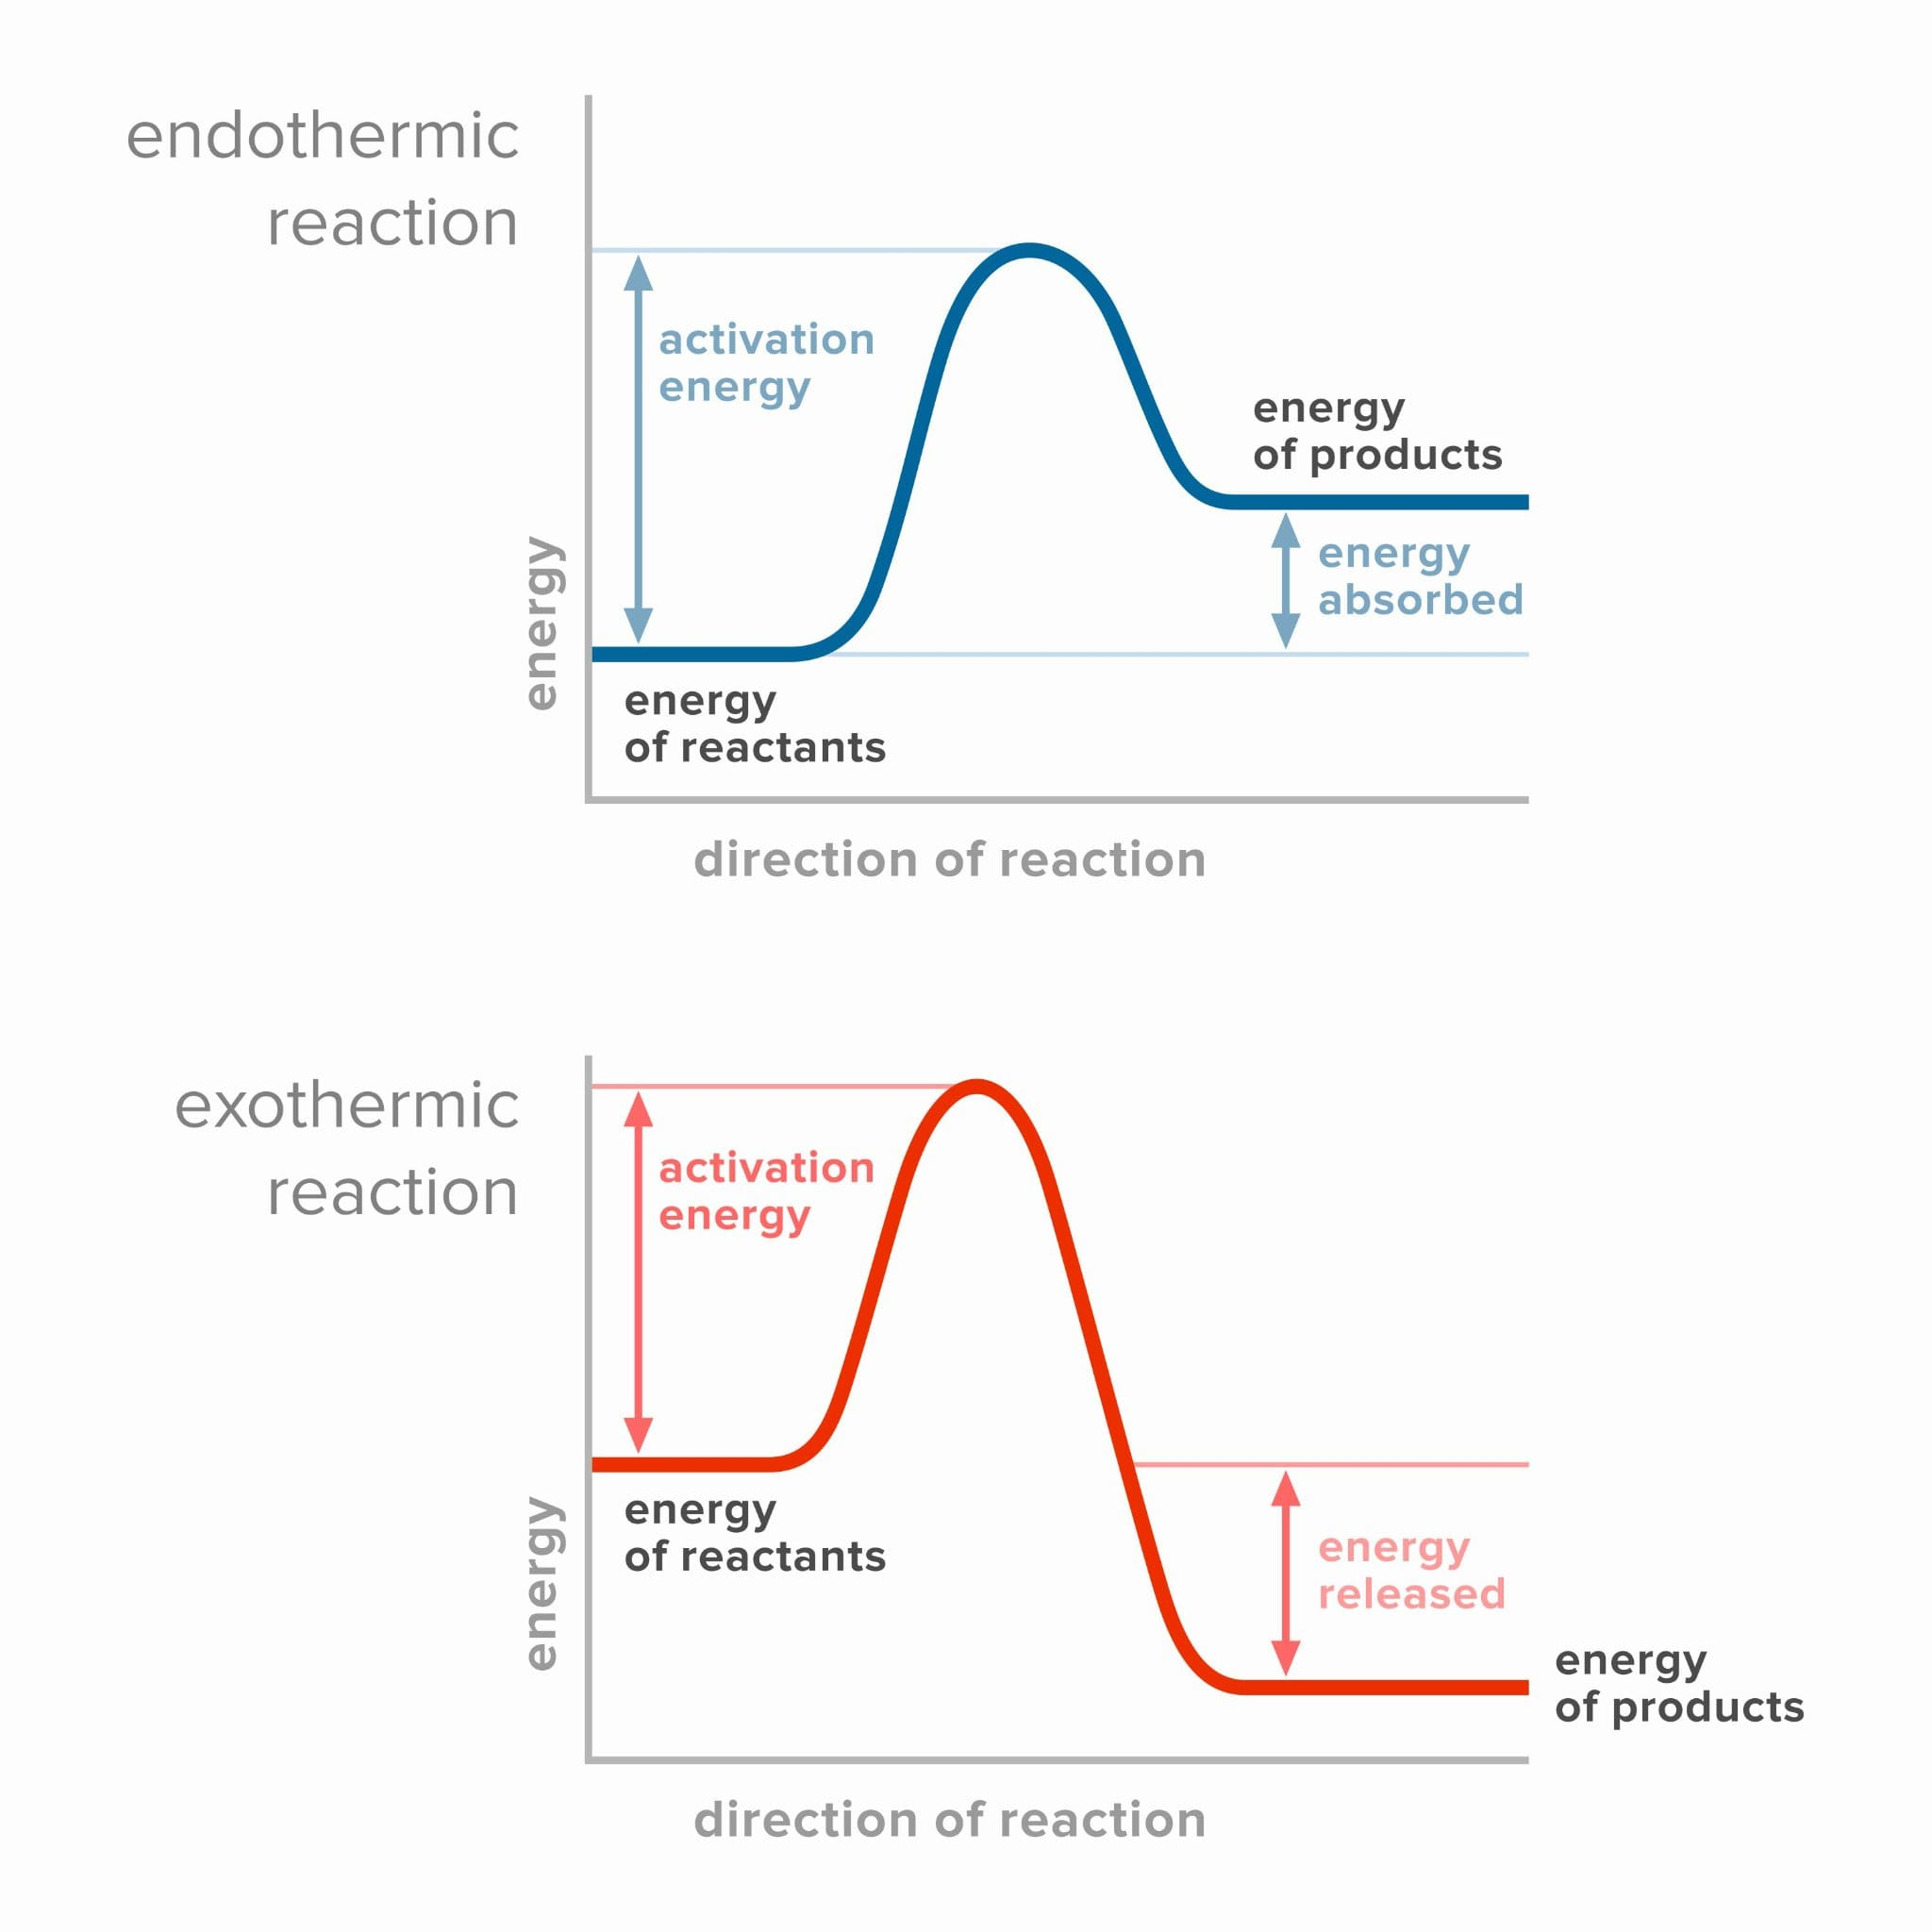
\includegraphics[width=0.6\textwidth]{eldiag.jpg}
\end{figure}

Activation energy, or \(E_a\), is the energy required to undergo a specific reaction. Energy released/absorbed is denoted by \(\Delta H\).

\subsection*{Heat Transfer}

\begin{equation}\label{heattransfer}
q = mc \Delta T
\end{equation}
where:
\begin{itemize}[leftmargin=*, nosep]
\item $q$ is heat in joules
\item $m$ is mass in grams
\item $c$ is the specific heat capacity in joules over degrees Celsius
\item $\Delta T$ is the change in temperature in degrees Celsius or Kelvin
\end{itemize}

\subsubsection*{Heat Units}

1 kilocalorie/food calorie (kcal or Cal) = 1000 calories (cal) = 4184 joules (J)

\subsection*{Heat Curves}
A heat curve for water:\footnote{This is hand-drawn because I have not yet mastered the art of TikZ. Maybe soon?}

\begin{figure}[H]
\centering
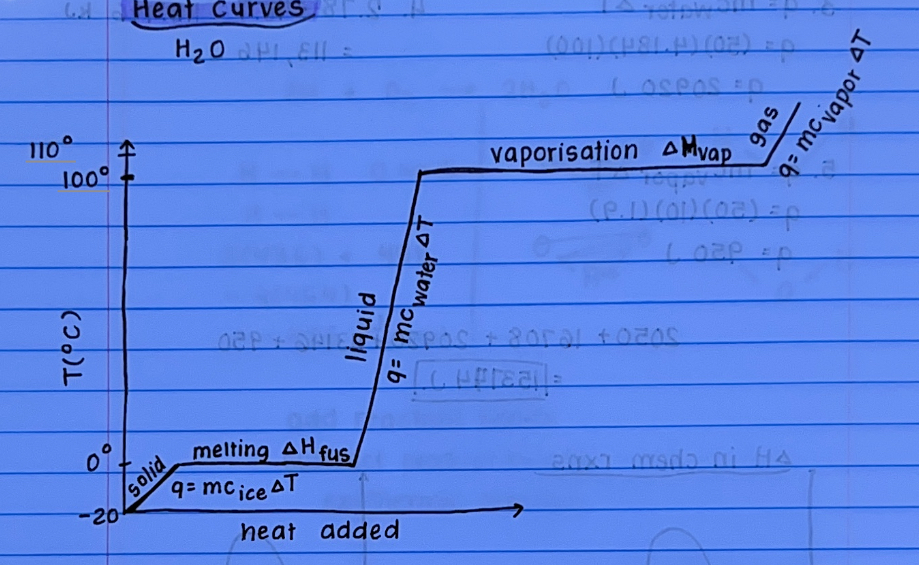
\includegraphics[width=0.7\textwidth]{heatcurve.jpg}
\end{figure}

$\Delta H_\text{fusion}$: amt of heat/mol that is absorbed when melting or released when freezing
$\Delta H_\text{vapor}$: amt of heat/mol absorbed when vaporising/released when condensing

Example: How much heat does it take to change 50 $g$ of water from a solid state at -20 \degC to a vapor state at 110 \degC?

Given:

\begin{itemize}[leftmargin=*, nosep]
	\item melting point of water: 0 \degC
	\item boiling point of water: 100 \degC
	\item $c_\text{ice}$ = 2.05 \cunits
	\item $c_\text{water}$ = 4.814 \cunits
	\item $c_\text{vapor}$ = 1.9 \cunits
	\item $\Delta H_\text{fus}$ = 6.01 $\frac{kJ}{mol}$
	\item $\Delta H_\text{vap}$ = 40.7 $\frac{kJ}{mol}$
\end{itemize}

This solution takes five steps. At the end, add them all together.

\textcolor{blue}{\textbf{Step 1:} Solid state.} The melting point of water is 0 \degC and the $\Delta T$ is 20. Use \(q = mc_\text{ice}\Delta T\):

\[q = (50)(2.05)(20) = 2050 \: J\]

\textcolor{blue}{\textbf{Step 2:} Fusion (melting).} By a simple calculation, we can find that there are 2.78 $mol$ of water. Convert to kilojoules, then to joules:

\[6.01 \: \frac{kJ}{mol} \cdot 2.78 \: mol = 16.708 \: kJ = 16708 \: J\]

\textcolor{blue}{\textbf{Step 3:} Liquid state.} The boiling point of water is 100 \degC and the $\Delta T$ is 100. Use \(q = mc_\text{water}\Delta T\):

\[q = (50)(4.184)(100) = 20920 \: J\]

\textcolor{blue}{\textbf{Step 2:} Vaporisation (boiling).} Using the same 2.78 $mol$ of water, convert $\Delta H_\text{vap}$ to kilojoules, then to joules:

\[40.7 \: \frac{kJ}{mol} \cdot 2.78 \: mol = 113.146 \: kJ = 113146 \: J\]

\textcolor{blue}{\textbf{Step 5:} Vapor state.} The final temperature is 110 \degC and the $\Delta T$ is 10. Use \(q = mc_\text{vapor}\Delta T\):

\[q = (50)(1.9)(10) = 950 \: J\]

\textcolor{blue}{\textbf{Step 6:} Add each change in heat together.}

\[2050 + 16708 + 20920 + 113146 + 950\]
\[=\boxed{153774 \: J}\]

\subsection*{$\Delta H$ in Reactions}
Breaking bonds \textbf{absorbs} heat, and making bonds \textbf{releases} heat. A positive $\Delta H$ suggests an endothermic reaction, and a negative $\Delta H$ suggests an exothermic reaction. To find the $\Delta H$ from a chemical equation, subtract the bond energies of the products from those of the reactants.

\subsection*{Hess' Law}
When adding reactions, you can also add $\Delta H$ values.

Example: Find the $\Delta H$ of the overall reaction.

$$\text{Overall rxn}: \text{CH}_{4(g)} + \text{H$_2$O}_{(g)} \longrightarrow \text{CO}_{(g)} + \text{3H}_{2(g)}$$
$$\text{CO}_{(g)} + \nicefrac12 \text{O}_{2(g)} \longrightarrow \text{CO}_{2(g)}, \Delta H = -283 \: \frac{kJ}{mol}$$
$$\text{H}_{2(g)} + \nicefrac12 \text{O}_{2(g)} \longrightarrow \text{H$_2$O}_{(g)}, \Delta H = -242 \: \frac{kJ}{mol}$$
$$\text{CH}_{4(g)} + \text{2O}_{2(g)} \longrightarrow \text{CO}_{2(g)} + \text{2H$_2$O}_{(g)}, \Delta H = -803 \: \frac{kJ}{mol}$$

Manipulate the three equations so that all the unnecessary elements cancel out:

$$\text{Flip}: \cancel{\text{CO}_{2(g)}} \longrightarrow \text{CO}_{(g)} + \cancel{\nicefrac12 \text{O}_{2(g)}}, \Delta H = 283 \: \frac{kJ}{mol}$$
$$\text{Flip and multiply by 3}: \cancel{\text{3H$_2$O}_{(g)}} \text{H$_2$O}_{(g)} \longrightarrow \text{3H}_{2(g)} + \cancel{\nicefrac32 \text{O}_{2(g)}}, \Delta H = 726 \: \frac{kJ}{mol}$$
$$\text{Leave as is}: \text{CH}_{4(g)} + \cancel{\text{2O}_{2(g)}} \longrightarrow \cancel{\text{CO}_{2(g)}} + \cancel{\text{2H$_2$O}_{(g)}}, \Delta H = -803 \: \frac{kJ}{mol}$$

Leaving us with the overall reaction:

$$\text{CH}_{4(g)} + \text{H$_2$O}_{(g)} \longrightarrow \text{CO}_{(g)} + \text{3H}_{2(g)}$$

Adding the $\Delta H$ values:

$$283 + 726 - 803$$
$$ = \boxed{206 \: \frac{kJ}{mol}.}$$

\end{document}
